\chapter{Ottimizzazione}
Nel corso di Machine Learning abbiamo conosciuto il \textbf{Stochastic Gradient Descent}, ma anche alcune delle sue varianti (Batch e MiniBatch), un meccanismo attraverso il quale si va a ricercare delle condizioni di ottimalità. In questo capitolo affronteremo proprio i problemi legati all'\textbf{Ottimizzazione} e le tecniche che hanno portato all'evoluzione e la modifica della classica discesa del gradiente. Ogni modello è caratterizzato da parametri (pesi e bias), essi determinano come il modello sia in grado di trasformare gli input in output. L'obbiettivo del processo di apprendimento risulta essere quello di trovare valori dei pesi che minimizzino l'errore. La superficie d'errore (Figura~\ref{fig:error_surface}), è una rappresentazione grafica di come la funzione di costo varia al modificarsi dei pesi.

\begin{figure}[h]
\centering
\includegraphics[width=0.5\textwidth]{figure/error_surface.png}
\caption{L’immagine illustra la "mappa" della funzione d’errore. Con una rappresentazione dell'errore rispetto a un peso in cui si mostra l'andamento parabolico, e il suo valore ottimizzato è il vertice (sopra). Ma anche la rappresentazione rispetto a due pesi, dove il valore ottimizzato si trova al centro delle ellissi, ognuna delle quali è una curva di livello (sotto).}
\label{fig:error_surface}
\end{figure}

\section{Discesa del Gradiente}
La discesa del gradiente (gradient descent) è l’algoritmo che usiamo per muoverci su questa superficie e raggiungere il punto di errore minimo. Immagina una pallina che rotola sulla superficie, all’inizio si trova in un punto alto (errore grande). Ad ogni passo, si muove nella direzione in cui la pendenza scende più rapidamente (cioè la direzione del gradiente negativo), essa continuerà a scendere fino ad arrivare in fondo alla "valle" della superficie, dove la pendenza è zero (minimo locale o globale). Questa discesa si concretizza con l'aggiornamento continuo dei pesi nel seguente modo:

\begin{equation}
    w_i^{(t+1)} =w_i^{(t)}-\eta\frac{\partial E}{\partial w_i}
\end{equation}

Una considerazione da effettuare è misurare con quanta velocità giungiamo alla "valle" durante la nostra discesa, questa carattiristica può variare a seconda del valore assegnato al Learning Rate ($\eta$), pertanto conviene sceglierlo in maniera opportuna.

\subsection{Scegliere il learning rate}
Per poter scegliere il learning rate, si inizia solitamente impostandolo a un valore elevato, per far si che si eviti di collassare all'interno di un minimo locale troppo presto (il nostro obbiettivo è giungere al minimo globale). Successivamente, attraverso tecniche di decadimento (decay), lo riduciamo progressivamente per aumentare la probabilità di convergere verso un minimo globale o comunque, un minimo locale migliore rispetto a quelli precedenti. Tra le strategie più comuni per il decadimento del learning rate possiamo considerare le seguenti:
\begin{itemize}
\item\textbf{Step Decay:} il learning rate viene ridotto di un fattore fisso dopo un certo numero di epoche;
\item\textbf{Exponential Decay:} il learning rate diminuisce esponenzialmente nel tempo;
\item\textbf{Adaptive Learning Rate:} tecniche come Adam e RMSprop regolano dinamicamente, adattando il learning rate per ogni parametro della rete.
\end{itemize}

\begin{figure}[!ht]
    \centering
    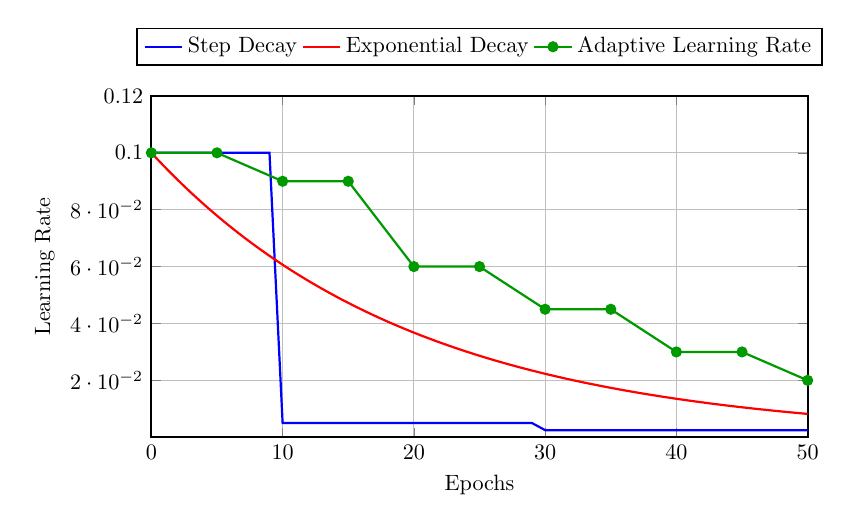
\begin{tikzpicture}[scale=0.8]
        \begin{axis}[
            width=12cm, height=7cm,
            xlabel={Epochs},
            ylabel={Learning Rate},
            xmin=0, xmax=50,
            ymin=0, ymax=0.12,
            legend style={
                at={(0.5,1.2)},
                anchor=north,
                legend columns=3
            },
            xtick={0,10,20,30,40,50},
            ytick={0.02,0.04,0.06,0.08,0.1,0.12},
            grid=both,
            thick,
            every axis plot/.append style={line width=1pt},
        ]

        % Step decay
        \addplot[blue, domain=0:50, samples=51] 
            {0.1 * (x<10 ? 1 : (x<30 ? 0.05 : 0.025))};
        \addlegendentry{Step Decay}

        % Exponential decay
        \addplot[red, domain=0:50, samples=200]
            {0.1 * exp(-0.05*x)};
        \addlegendentry{Exponential Decay}

        % Adaptive (manually simulated)
        \addplot[green!60!black, mark=*] 
            coordinates {
                (0, 0.1) (5, 0.1) (10, 0.09) (15, 0.09)
                (20, 0.06) (25, 0.06) (30, 0.045)
                (35, 0.045) (40, 0.03) (45, 0.03) (50, 0.02)
            };
        \addlegendentry{Adaptive Learning Rate}

        \end{axis}
    \end{tikzpicture}
    \caption{Confronto tra diverse strategie di decadimento del learning rate.}
    \label{fig:lr_decay}
\end{figure}

\subsection{Inizializzazione dei pesi}
Oltre al valore del Learning Rate, è cruciale inizializzare i pesi delle reti neurali in maniera opportuna. A differenza della regressione lineare in cui l'ottimizzazione è diretta, nelle reti neurali l'algoritmo di backpropagation può essere compromesso nel caso in cui i pesi della nostra rete non siano scelti accuratamente. 

\begin{Osservazione}
    Se due pesi all'interno di uno stesso layer hanno lo stesso valore iniziale, l'errore propagato all'indietro attraverso la rete, genererà gli stessi aggiornamenti, impedendo alla rete di apprendere in maniera corretta.
\end{Osservazione}

\begin{Osservazione}
    Qual'ora i pesi vengano inizializzati con valori troppo grandi, riscontreremo una possibilità di esplosione della rete neurale.
\end{Osservazione}

\begin{Osservazione}
    Se i pesi vengono inizializzati con valori troppo piccoli, potremmo incorrere in una possibile scomparsa del valore del gradiente.
\end{Osservazione}

Oltre tutte queste osservazioni, si potrebbe incorrere banalmente in una non convergenze, generando il fenomeno dell'Overshoot, in cui il gradiente oscilla in continuazione da una parte all'altra del valore minimo a cui si dovrebbe convergere.

\subsection{Xavier Glorot Initialization}
\marginpar{\href{https://proceedings.mlr.press/v9/glorot10a/glorot10a.pdf}{"Understanding the difficulty of training deep feedforward neural networks" by Xavier Glorot et al. (2010)~\cite{glorot2010understanding}}}
Prima di inoltrarci nel metodo di Inizializzazione studiato da Xavier~\cite{glorot2010understanding}, è necessario affrontare delle definizioni importanti.

\begin{Definizione}[Fan-in]
    Il Fan-in è il numero di neuroni che alimentano un neurone nel layer successivo;
\end{Definizione}

\begin{Definizione}[Fan-out]
    Il Fan-out è il numero di neuroni che un dato neurone alimenta nel layer successivo;
\end{Definizione}

\begin{Esempio}
    Consideriamo un layer completamente connesso (fully connected, FC) con: 256 neuroni in ingresso e 512 neuroni in uscita, il suo fan-in sarà 256 e il suo fan-out sarà pari a 512.
\end{Esempio}

Tecniche come quella studiata da Xavier Glorot prendono in considerazione questi aspetti, utilizzando distribuzioni gaussiane o uniformi adeguate da cui pescare i valori dei pesi, invece di pensare a un'inizializzazione casuale. L’idea chiave di questa inizializzazione conosciuta come \textbf{Xavier} è scegliere i pesi in modo tale che vengano soddisfatte le due seguenti proprietà:
\begin{enumerate}
    \item La varianza dell'output di un neurone sia simile alla varianza del suo input;
    \item La varianza dei gradienti rimanga costante tra gli strati;
\end{enumerate}

In parole povere, si cerca di mantenere l'energia del segnale costante mentre attraversa la rete, sia in avanti che all'indietro. Per ottenere questo risultato, i pesi di ogni strato vengono estratti casualmente da una distribuzione (solitamente uniforme o normale) con una media nulla e una varianza specifica, nel caso della distribuzione normale, calcolata in base al numero di Fan-in e di Fan-out. Il valore della varianza solitamente è uno dei due:

\begin{equation}
    \operatorname{Var}(W) = \frac{1}{n_{in}}\quad \text{o}\quad \operatorname{Var}(W)= \frac{2}{n_{in}+n_{out}}
\end{equation}

\begin{Osservazione}
    Nelle slide del Professor Anelli, la seconda formula compare con un 1 al numeratore, questa non risulta essere sbagliata in senso assoluto, ma sono due varianti della stessa idea, quella che è riportata qui si basa sul paper ufficiale~\cite{glorot2010understanding}, in cui si adotta una media armonica tra i due requisiti, differentemente da quella presente nelle slide la quale adotta la media aritmetica.
\end{Osservazione}

Utilizzando una distribuzione uniforme la formula sarà la seguente:
\begin{equation}
    \mathcal{U}\left(-\frac{\sqrt{6}}{\sqrt{n_{in}+n_{out}}},\,\frac{\sqrt{6}}{\sqrt{n_{in}+n_{out}}}\right)
\end{equation}

La Xavier Initialization risulta essere un miglioramento rispetto all'inizializzazione a zero o quella casuale arbitraria, perché bilancia la propagazione del segnale nei vari strati. In ogni caso non risulta essere sempre ideale per funzioni di attivazione non lineari come ReLU, per cui esiste una variante chiamata \textit{He initialization} che utilizza un 2 al numeratore nella distribuzione gaussiana.

\subsection{Normalizzazione}
Per normalizzare i dati, possiamo utilizzare tecniche come la \textit{min-max normalization} e la \textit{z-score normalization}, già viste nel corso di Machine Learning, esse rendono il dataset più coerente e scalabile. Il problema di queste tecniche, però è che effettuano un'assunzione quasi mai vera, ossia che le feature sia scorrelate fra loro. Pertanto la sfida passa ad effettuare una decorrelazione delle feature in modo efficace, risultato ottenibile in diversi modi:
\begin{itemize}
\item\textbf{Principal Component Analysis (PCA):} tecnica che trasforma le feature originali in nuove variabili non correlate;
\item\textbf{Whitening:} trasformazione che rende le feature scorrelate con varianza unitaria;
\item\textbf{Batch Normalization:} tecnica che normalizza le attivazioni durante l'addestramento per migliorare la stabilità e accelerarne la convergenza.
\end{itemize}

\begin{table}[!ht]
    \centering
    \caption{Confronto tra PCA, Whitening e Batch Normalization}
    \begin{adjustbox}{width=\textwidth}
    \begin{tabular}{@{} lccc @{}}
        \toprule
        \textbf{Caratteristica} & \textbf{PCA} & \textbf{Whitening} & \textbf{Batch Normalization} \\
        \midrule
        \textbf{Tipo} & Preprocessing & Preprocessing & In-training normalizzazione \\
        \textbf{Obiettivo} & Riduzione dimensionalità & Decorrelazione delle feature & Accelerare il training \\
        \textbf{Agisce su} & Intero dataset & Intero dataset & Mini-batch durante il training \\
        \textbf{Rende varianza uniforme?} & No & Sì (varianza unitaria) & No (mantiene varianza originale) \\
        \textbf{Rende feature ortogonali?} & Sì & Sì & No \\
        \textbf{Mantiene struttura dati?} & Parzialmente & Meno rispetto a PCA & Sì \\
        \textbf{Uso tipico} & Compressione dati, pretraining & Preprocessing per ICA, SVM & Normalizzazione nei layer di Reti Neurali \\
        \textbf{Effetto su reti neurali} & Riduce dimensionalità in input & Raramente usato direttamente & Migliora stabilità e velocità di training \\
        \bottomrule
    \end{tabular}
    \end{adjustbox}
\end{table}

\section{Momentum}
L'algoritmo di discesa del gradiente rappresenta la base di gran parte dei metodi di ottimizzazione, nonostante la sua semplicità ed efficacia teorica, presenta alcune limitazioni pratiche, soprattutto in presenza di superfici di errore complesse e irregolari. Uno dei principali problemi riguarda la \textbf{velocità di convergenza} quando la funzione di costo assume una forma fortemente non uniforme, ossia caratterizzata da \textit{valli strette e lunghe}. In tali casi, la pendenza della funzione può risultare molto ripida in una direzione e quasi piatta in un'altra. Di conseguenza, il vettore gradiente, che indica la direzione di massima variazione dell'errore, non punta direttamente verso il minimo, ma tende ad alternarsi tra le direzioni di massima e minima pendenza. Questo comportamento provoca una \textbf{traiettoria oscillatoria} nel processo di aggiornamento dei pesi: il modello si muove rapidamente lungo la direzione ripida, mentre procede molto lentamente lungo quella piatta. Il risultato è una convergenza rallentata, proprio come se ci trovassimo fra due pareti rocciose molto ripide e man mano che scendiamo lungo un canale che è la direzione desiderata, andassimo a sbattere alle due pareti. Per mitigare tali effetti, sono stati introdotti ottimizzatori più avanzati che estendono la discesa del gradiente classica. Tra questi, il metodo del \textbf{Momentum} riduce le oscillazioni accumulando una componente inerziale nella direzione di discesa, basandosi sulla storia dei gradienti precedenti smorzando le oscillazioni.

%mentre approcci adattivi come \textbf{AdaGrad}, \textbf{RMSProp} e \textbf{Adam} regolano dinamicamente l'ampiezza dei passi di aggiornamento per ciascun parametro, accelerando la convergenza nelle direzioni piatte e stabilizzandola in quelle più ripide.

\begin{equation}
    \left\{\begin{array}{c}
    v_{t} = \beta v_{t-1} - \eta\,\nabla J(w_t)
    \\
    w_{t+1} = w_t + \,v_{t}
    \end{array}\right.
\end{equation}
\\
In questo caso $v$ sarebbe il \textit{Momentum Parameter} il quale prende in analisi la velocità di discesa fino a un determinato momento, mentre $\beta$ è il così detto \textit{Damping Factor}, un valore che controlla quanto la velocità passata influenza quella attuale, compreso fra zero e uno, se fosse zero, staremmo facendo semplicemente la discesa del gradiente, nel caso unitario invece avrei un'esplosione del gradiente nella nostra rete neurale. Il valore del damping factor, ci permette di capire la velocità del cambio di direzione in base, più sarà piccolo, più la direzione cambierà velocemente.

\begin{figure}[ht]
    \centering
    \includegraphics[width=\textwidth]{figure/DampingFactMomentum.png}
    \caption{Confronto delle traiettorie per diversi valori di $\beta$ nel Momentum}
\end{figure}

\section{Nesterov Accelerated Gradient}
Il Momentum classico aiuta la discesa del gradiente accelerando il processo e smorzando le oscillazioni, ma ha un problema: aggiorna i pesi basandosi sulla direzione del gradiente calcolato nella posizione attuale, senza considerare dove il peso si troverà dopo l'aggiornamento. Il matematico Yurii Nesterov nel 1983 propose una modifica al Momentum classico, chiamata \textbf{Nesterov Accelerated Gradient} (NAG), migliorando la velocità di convergenza e la stabilità dell’ottimizzazione. L'analogia per chiarire di cosa si tratta è immaginarsi una persona in bicicletta: nel momentum classico, la persona spinge sui pedali senza guardare avanti basandomi andando sempre più veloce. Se la strada curva improvvisamente, potrei andare troppo veloce nella direzione sbagliata e dover correggere bruscamente. Con il momentum di Nesterov, è come se guardassi avanti prima di spingere, capendo dove sto andando e valutando quanta forza imprimere sui pedali per correggere il movimento in base lla direzione da seguire.
\begin{figure}
    \centering
    \includegraphics[width=0.75\textwidth]{figure/momenest.png}
    \caption{Nel grafico è possibile vedere la velocità di convergenza confrontando i due Momentum entrambi partendo da uno stesso punto d'inizio, il Momentum classico come potevamo aspettarci avrà delle oscillazioni molto più grandi rispetto a quelle del Momentum di Nesterov.}
    \label{fig:MomentumVS}
\end{figure}
Il Momentum di Nesterov è più efficiente calcolando il gradiente in una posizione successiva vedendo in anticipo dove ci porterà la velocità calcolata, e calcolando il gradiente non nel punto attuale ma in quello anticipato, mantenendo così un'alta velocità senza instabilità.

\begin{equation}
\left\{\begin{array}{c}
    v_{t} = \beta v_{t-1}\,-\,\eta\,\frac{\partial J}{\partial(w_t\,+\,\beta\,v_{t-1})}\\
    w_{t+1} = w_t\,+\,v_t
    \end{array}\right.
\end{equation}

Nesterov è un piccolo ma potente miglioramento rispetto al Momentum classico. Questo metodo viene spesso usato negli ottimizzatori moderni come Adam, RMSprop con Momentum, e molte varianti di SGD, perché migliora stabilità e velocità di convergenza.

\subsection{Ma perché proprio funziona il Momentum ?}
Il Momentum funziona principalmente per due motivi:
\begin{enumerate}
    \item Accelerazione dell'ottimizzazione;
    \item Attenuazione del rumore;
\end{enumerate}

\subsubsection{Accelerazione dell'ottimizzazione}
L'idea del momentum è come spingere un carrello in discesa, se do un piccolo colpo, esso si muoverà piano, se continuo a spingere il carrello guadagnerà velocità, e qual'ora smettessi di spingere, continuerà a muoversi per inerzia. Matematicamente questo viene aggiunto grazie all'aggiornamento dei pesi tramite l'utilizzo di un valore che tiene conto dei valori precedenti nel calcolo del gradiente. Pertanto se i gradienti puntano nella stessa direzione per più step, la velocità aumenta e il modello converge più velocemente.
\subsubsection{Attenuazione del rumore}
Con il Momentum, accumuliamo un valore mediato nel tempo, riducendo il rumore casuale come succedeva normalmente a ogni piccola variazione. Se il rumore nei gradienti punta in direzioni casuali, questi si annullano nel tempo, il movimento risulta più fluido e meno oscillante e infine permette di superare piccoli ostacoli senza rimanere bloccati in minimi locali poco profondi. Il Momentum di Nesterov, migliora ulteriormente entrambi gli aspetti anticipando il passo successivo prima di aggiornare la velocità, evitando così di andare troppo oltre e migliorando la precisione.
%%%%ARRIVATO QUI
\section{Learning Rate adattivo}
I parametri presenti in un modello, possono avere delle tipologie di scale di aggioranmento differenti, proprio per questo nasce l'idea di creare un \textbf{Learning Rate adattivo}. Nel momento in cui prendiamo una direzione di discesa al posto di un'altra, potremmo ritrovarci che ci siano richieste di un learning rate più grande o più piccolo, se ne usassimo uno fisso per tutti i parametri porterebbero a delle oscillazioni, o convergenze dilatate nel tempo. Quindi viene deciso di adattare il learning rate in modo indipendente per ogni parametro, basandosi sull'andamento del gradiente.

\subsection{Additive increase multiplicative decrease}
Adattare il learning rate individualmente per ogni peso con un piccolo incremento e un decremento moltiplicativo nasce per poter bilanciare due aspetti:
\begin{itemize}
    \item Nel caso in cui il gradiente fosse coerente in una direzione $\rightarrow$ Aumentiamo il learning rate per accelerare la convergenza;
    \item Nel caso in cui il gradiente cambia direzione frequentemente $\rightarrow$ Riduciamo il learning rate per evitare oscillazioni.
\end{itemize}

Questa tecnica è utilizzata in metodi come \textbf{Adadelta}, \textbf{Rprop} (Resilient Propagation) e alcune varianti di \textbf{Adam}, tutte tecnice che vedremo a breve. Il funzionamento è semplice: nel momento in cui valuto i singoli learning rate, se il gradiente mantiene la stessa direzione, aumento il valore del learning rate per fare passi più grandi, diversamente se cambia di segno, significa che stiamo oscillando troppo, perciò ridurremo il learning rate per stabilizzarlo.

\section{Resilient Propagation (Rprop)}

La \textbf{Resilient Propagation} (Rprop), introdotta da Riedmiller et al. 1993~\cite{RiedmillerBraun1993}, è un metodo di ottimizzazione che affronta una delle principali debolezze della discesa del gradiente: la dipendenza dalla magnitudine del gradiente. L'idea fondamentale consiste nel considerare unicamente il \textit{segno} del gradiente per determinare la direzione dell'aggiornamento, mentre la grandezza del passo di apprendimento viene adattata dinamicamente per ciascun peso in modo indipendente. Per ogni parametro $w_i$ si definisce un valore di aggiornamento $\Delta_i(t)$, regolato in base alla coerenza del segno del gradiente nel tempo:
\[
\Delta_i(t) =
\begin{cases}
\eta^+ \cdot \Delta_i(t-1), & \text{se } \frac{\partial E(t-1)}{\partial w_i} \cdot \frac{\partial E(t)}{\partial w_i} > 0 \\[6pt]
\eta^- \cdot \Delta_i(t-1), & \text{se } \frac{\partial E(t-1)}{\partial w_i} \cdot \frac{\partial E(t)}{\partial w_i} < 0 \\[6pt]
\Delta_i(t-1), & \text{altrimenti}
\end{cases}
\]
Solitamente $\eta^+$ e $\eta^-$ hanno un valore rispettivamente di $1.2$ e $0.5$, l'aggiornamento del peso avviene quindi come:
\[
w_i(t+1) = w_i(t) - \operatorname{sign}\!\left(\frac{\partial E(t)}{\partial w_i}\right) \cdot \Delta_i(t)
\]

In questo modo, ciascun peso dispone di un proprio tasso di apprendimento che cresce quando la direzione del gradiente è coerente, e diminuisce quando essa si inverte. Tale meccanismo permette di accelerare la convergenza nelle regioni piatte della funzione di costo e di ridurre le oscillazioni nelle zone di forte curvatura.

\section{RMSprop}

Dopo gli approcci basati su aggiornamenti indipendenti dei pesi, come la \textbf{Resilient Propagation}, la ricerca sull’ottimizzazione dei modelli neurali si è orientata verso metodi in grado di adattare dinamicamente il tasso di apprendimento in base al comportamento locale del gradiente. Uno dei risultati più efficaci in questa direzione è l’algoritmo \textbf{RMSprop} (\textit{Root Mean Square Propagation}), introdotto da Geoffrey Hinton nel 2012~\cite{TielemanHinton2012RMSprop}. L’obiettivo è quello di stabilizzare la discesa del gradiente adattando il passo di aggiornamento di ciascun parametro in funzione della sua storia recente di variazioni. L’algoritmo nasce come una modifica del metodo \textbf{AdaGrad}, che riduce progressivamente il learning rate accumulando la somma dei quadrati dei gradienti. Tale accumulo, tuttavia, tende a far decrescere eccessivamente il passo di apprendimento, rallentando o bloccando la convergenza nelle fasi successive dell’addestramento. Per evitare questo problema, RMSprop introduce una \textit{media mobile esponenziale} dei quadrati dei gradienti, in modo da mantenere un bilanciamento costante tra memoria storica e reattività alle variazioni recenti. Formalmente, il valore medio viene aggiornato secondo:
\[
E[g^2]_t = \gamma E[g^2]_{t-1} + (1 - \gamma) (\nabla E(w_t))^2
\]
dove $\gamma$ rappresenta il fattore di decadimento (tipicamente pari a 0.9) e $\nabla E(w_t)$ è il gradiente calcolato al passo $t$. L’aggiornamento dei pesi diventa quindi:
\[
w_{t+1} = w_t - \frac{\eta}{\sqrt{E[g^2]_t + \epsilon}} \, \nabla E(w_t)
\]
dove $\eta$ è il learning rate e $\epsilon$ è una piccola costante per evitare divisioni per zero. In questo modo, ciascun parametro dispone di un proprio passo di apprendimento adattivo:  
\begin{itemize}
    \item Se un peso riceve gradienti di grande ampiezza, il termine $E[g^2]_t$ cresce e il passo viene ridotto, prevenendo oscillazioni e instabilità;
    \item Se i gradienti risultano piccoli o irregolari, il passo resta più ampio, accelerando la convergenza.
\end{itemize}

RMSprop si distingue quindi come una strategia di ottimizzazione \textit{localmente adattiva}, capace di bilanciare velocità e stabilità. Essa rappresenta il punto di transizione naturale tra i metodi a passo variabile per singolo parametro, come Rprop, e le tecniche completamente adattive di generazione successiva, come \textbf{AdaGrad}, che approfondiremo nella sezione seguente.


\section{AdaGrad}

L’algoritmo \textbf{AdaGrad} (\textit{Adaptive Gradient}) rappresenta uno dei primi approcci di ottimizzazione realmente \textit{adattivi}, introdotto da Duchi et al. 2011~\cite{DuchiHazanSinger2011AdaGrad}. La sua idea di fondo è quella di modificare dinamicamente il tasso di apprendimento per ciascun parametro del modello, in modo da rendere l’aggiornamento più sensibile alla frequenza e all’intensità dei gradienti associati a ogni peso. Nella discesa del gradiente tradizionale, un singolo valore di \textit{learning rate} $\eta$ viene applicato uniformemente a tutti i pesi. Tuttavia, i diversi parametri di una rete neurale possono contribuire in misura molto diversa alla funzione di costo: alcuni ricevono gradienti ampi e frequenti, altri piccoli o sporadici. AdaGrad affronta questo problema regolando automaticamente l’ampiezza del passo per ciascun peso in modo inversamente proporzionale alla somma cumulativa dei suoi gradienti al quadrato. Formalmente, si definisce per ogni parametro $w_i$ un accumulatore $G_i(t)$:
\[
G_i(t) = \sum_{k=1}^{t} \left( \frac{\partial E(w_i^{(k)})}{\partial w_i} \right)^2
\]
e l’aggiornamento dei pesi avviene come:
\[
w_i^{(t+1)} = w_i^{(t)} - \frac{\eta}{\sqrt{G_i(t) + \epsilon}} \, \frac{\partial E(w_i^{(t)})}{\partial w_i}
\]
dove $\epsilon$ è una piccola costante di stabilità numerica. In questo modo, i parametri che ricevono gradienti grandi in modo persistente avranno un denominatore più elevato e quindi un passo di aggiornamento più piccolo; viceversa, quelli con gradienti rari o deboli verranno aggiornati con passi più ampi. Il risultato è un comportamento di \textbf{auto-regolazione locale del learning rate} che tende a migliorare la convergenza. Tuttavia, la caratteristica di AdaGrad di accumulare indefinitamente il quadrato dei gradienti comporta un effetto collaterale significativo: con il progredire dell’addestramento, $G_i(t)$ cresce costantemente, facendo diminuire il learning rate effettivo fino a valori prossimi allo zero.  
Ciò può portare a un \textbf{prematuro rallentamento della convergenza}, specialmente nelle fasi finali dell’ottimizzazione, quando il modello necessiterebbe ancora di piccoli aggiustamenti. Per ovviare a tale problema, sono state introdotte varianti più flessibili, come la \textbf{Adadelta}, che mantiene l’adattività di AdaGrad ma sostituisce la somma cumulativa con una media mobile esponenziale dei gradienti al quadrato, preservando così un equilibrio più stabile nel tempo. Nella sezione seguente analizzeremo in dettaglio il funzionamento di questo approccio.

\section{Adadelta}

L’algoritmo \textbf{Adadelta}, proposto da Zeiler nel 2012~\cite{Zeiler2012AdaDelta}, nasce come evoluzione diretta di \textbf{AdaGrad}, con l’obiettivo di risolvere il problema del decadimento eccessivo del tasso di apprendimento dovuto all’accumulo cumulativo dei gradienti al quadrato. Come visto nella sezione precedente, AdaGrad tende infatti a ridurre progressivamente il learning rate fino quasi ad annullarlo, ostacolando la capacità del modello di continuare ad apprendere nelle fasi avanzate dell’addestramento. L’idea di Adadelta è di sostituire la somma cumulativa con una \textbf{media mobile esponenziale} dei gradienti al quadrato, mantenendo così una memoria a breve termine della loro variazione. In questo modo, l’algoritmo conserva la natura adattiva di AdaGrad, ma ne elimina il rallentamento asintotico. Formalmente, per ciascun parametro $w_i$, la media mobile viene aggiornata secondo:
\[
E[g_i^2]_t = \rho E[g_i^2]_{t-1} + (1 - \rho) \left( \frac{\partial E(w_i^{(t)})}{\partial w_i} \right)^2
\]
dove $\rho$ è il fattore di decadimento esponenziale (tipicamente compreso tra 0.9 e 0.95). L’ampiezza del passo viene poi calcolata come:
\[
\Delta w_i^{(t)} = - \frac{\sqrt{E[\Delta w_i^2]_{t-1} + \epsilon}}{\sqrt{E[g_i^2]_t + \epsilon}} \, \frac{\partial E(w_i^{(t)})}{\partial w_i}
\]
e infine i pesi vengono aggiornati come:
\[
w_i^{(t+1)} = w_i^{(t)} + \Delta w_i^{(t)}
\]

Un aspetto distintivo di Adadelta è l’introduzione di una seconda media mobile $E[\Delta w_i^2]_t$, che tiene traccia dell’ampiezza media degli aggiornamenti precedenti. Questo termine funge da \textbf{meccanismo di autoregolazione del passo}, consentendo all’algoritmo di adattare dinamicamente non solo la direzione, ma anche la scala delle variazioni dei pesi. Il risultato è un comportamento più stabile e coerente, che non richiede l’impostazione manuale di un learning rate globale. Grazie a queste caratteristiche, Adadelta è particolarmente efficace in scenari in cui i gradienti variano in modo non uniforme o decrescono rapidamente nel tempo. Il metodo può essere interpretato come un ponte concettuale tra AdaGrad e gli ottimizzatori successivi come \textbf{RMSprop} e \textbf{Adam}, che ne erediteranno il principio di adattività locale combinandolo con ulteriori strategie di momentum e media mobile dei gradienti. In sintesi, Adadelta rappresenta un passo fondamentale nell’evoluzione degli algoritmi di ottimizzazione, poiché introduce una forma di apprendimento adattivo completamente autonoma, in grado di bilanciare efficacemente velocità di convergenza e stabilità numerica senza dipendere da un tasso di apprendimento fisso.

\section{Adam}

L’algoritmo \textbf{Adam} (\textit{Adaptive Moment Estimation}), proposto da Kingma et al. 2015~\cite{KingmaBa2015Adam}, rappresenta una delle più efficaci e diffuse tecniche di ottimizzazione nel deep learning moderno. Adam combina i principi del \textbf{momentum} e dei metodi \textbf{adattivi} come \textbf{RMSprop}, fornendo un aggiornamento dei pesi che è allo stesso tempo stabile, veloce e robusto rispetto alle variazioni della scala dei gradienti. L’idea centrale consiste nel mantenere due medie mobili esponenziali:
\begin{itemize}
    \item Una per la \textbf{stima del primo momento} (la media dei gradienti), analoga al momentum classico;
    \item Una per la \textbf{stima del secondo momento} (la media dei quadrati dei gradienti), come in RMSprop.
\end{itemize}

Formalmente, per ciascun parametro $w_i$, al passo $t$ si definiscono:
\[
m_t = \beta_1 m_{t-1} + (1 - \beta_1) \nabla E(w_t)
\]
\[
v_t = \beta_2 v_{t-1} + (1 - \beta_2) (\nabla E(w_t))^2
\]
dove:
\begin{itemize}
    \item $m_t$ rappresenta la stima del primo momento (velocità media),
    \item $v_t$ rappresenta la stima del secondo momento (varianza),
    \item $\beta_1$ e $\beta_2$ sono coefficienti di decadimento esponenziale, tipicamente $\beta_1 = 0.9$ e $\beta_2 = 0.999$.
\end{itemize}

Poiché entrambe le stime vengono inizializzate a zero, Adam applica una correzione al bias introdotto dalle prime iterazioni:
\[
\hat{m}_t = \frac{m_t}{1 - \beta_1^t}, \qquad
\hat{v}_t = \frac{v_t}{1 - \beta_2^t}
\]
L’aggiornamento dei pesi avviene quindi secondo:
\[
w_{t+1} = w_t - \frac{\eta}{\sqrt{\hat{v}_t} + \epsilon} \, \hat{m}_t
\]
dove $\eta$ rappresenta il learning rate e $\epsilon$ è una costante di stabilità numerica (solitamente $10^{-8}$). Grazie a questa formulazione, Adam unisce:
\begin{itemize}
    \item La \textbf{stabilità} dei metodi basati su media mobile (come RMSprop), che riducono il passo nelle direzioni ad alta curvatura;
    \item La \textbf{velocità di convergenza} del momentum, che mantiene la direzione media di discesa evitando oscillazioni.
\end{itemize}

L’algoritmo si adatta automaticamente alla scala dei gradienti di ciascun parametro, eliminando la necessità di un tuning fine del learning rate e rendendolo particolarmente efficace in reti profonde o con dati rumorosi. Per questo motivo, Adam è oggi uno degli ottimizzatori di default in numerosi framework di deep learning e architetture moderne (Transformer, GAN, reti convoluzionali, ecc.).

\subsection{Limitazioni di Adam}
Adam non è perfetto, esso incorre in alcune limitazioni:
\begin{itemize}
    \item\textbf{Sovra-adattamento ai dati rumorosi}: Adam si adatta velocemente, ma può reagire troppo a gradienti rumorosi, riducendo la capacità del modello di generalizzare bene;
    \item \textbf{Decay inefficace del peso}: Adam non fa un vero weight decay come la discesa del gradiente classica. Nel SGD viene incluso il parametro di regolarizzazione, questa cosa viene effettuata in Adam, nel learning rate adattivo, dunque è meno efficace;
    \item\textbf{Rallentata convergenza finale}:Adam spesso converge rapidamente all'inizio, ma poi rallenta molto nel trovare il minimo ottimale. Questo poiché i learning rate adattivi riducono troppo la velocità di aggiornamento nelle fasi finali.
\end{itemize}
Per mitigare tale comportamento, è stata introdotta una variante più stabile nota come \textbf{AdamW}.
\begin{figure}
    \centering
    \includegraphics[width=0.7\textwidth]{figure/sgrmspropadam.png}
    \caption{Grafico che mette in luce le differenze nella convergenza fra lo SGD, la RMSprop e Adam}
    \label{fig:diffAdamSGDRMSprop}
\end{figure}

\subsection{AdamW}

L’ottimizzatore \textbf{AdamW} (\emph{Adam with Weight Decay}), proposto da Loshchilov et al. 2017~\cite{LoshchilovHutter2017AdamW}, modifica la regolarizzazione di Adam separando esplicitamente il termine di \textit{weight decay} dall’aggiornamento del gradiente. Nel metodo Adam classico, la penalizzazione $L_2$ sui pesi viene incorporata nel gradiente stesso, alterando le medie mobili e introducendo interazioni indesiderate con il meccanismo adattivo. AdamW rimuove questa interferenza applicando il decadimento dei pesi come un’operazione separata:
\[
w_{t+1} = w_t - \eta \lambda w_t - \frac{\eta}{\sqrt{\hat{v}_t} + \epsilon} \, \hat{m}_t
\]
dove $\lambda$ è il coefficiente di \emph{weight decay}. Questa semplice modifica migliora la \textbf{generalizzazione} e la \textbf{stabilità numerica}, specialmente nei contesti di addestramento di grandi modelli come BERT e GPT. AdamW è oggi la variante di riferimento dell’ottimizzatore Adam ed è implementato come impostazione predefinita nei principali framework di deep learning.

\section{Lion}
Adam è l'ottimizzatore più utilizzato, nonostante ciò, non è il migliore, infatti nel Febbraio del 2023, è stato proposto un ottimizzatore completamente diverso da quelli precedenti, questo perché era stato proposto da un Agente di Intelligenza Artificiale. Crearlo tramite un calcolatore, ha portato a raffinare le formule trasportandole direttamente in linee di codice, considerandone l'impatto sul costo computazionale. Per rendere più compatto il codice, l'agente ha introdotto una funzione che è esattamente quella presente in tutti gli ottimizzatori che abbiamo visto fin'ora (funzione di interpolazione). Questo algoritmo permette di analizzarne vari, migliorati nei vari cicli di aggiornamento, effettuando un torneo fra loro, per combinare i migliori e generarne dei figli adottando i pregi dei genitori, raffinandosi sempre più, esattamente come accade con le manipolazioni genetiche. Di seguito il codice implementativo di Lion:

\begin{python}[frame=trBL] 
    def train(weight, gradient, momentum, lr): 
        update = interp(gradient, momentum, (*@$\beta_1$@*)) 
        update = sign(update) 
        momentum = interp(gradient, momentum, (*@$\beta_2$@*))
        weight_decay = weight * (*@$\lambda$@*) 
        update = update + weight_decay 
        update = update * lr 
    return update, momentum 
\end{python}

\section{Gradiente e Curvatura}
Nel momento in cui scegliamo la direzione in cui convergere, bisognerebbe chiedersi di quanto diminuisca l'errore prima di ricomonciare a salire, solitamente noi assumiamo che la curvatura sia costante, cioè che si tratti di una superficie di errore quadratica, assumiamo nella nostra analisi che l'entità del gradiente diminuisca man mano che ci spostiamo verso il basso, la riduzione massima dell'errore dipende dal rapporto fra il gradiente e la curvatura, e una buona direzione nella quale è efficiente muoversi è quella con un elevato rapporto fra gradiente e curvatura, pertanto il giusto interrogativo da porsi è come trovare il giusto valore del rapporto.

\section{Metodo di Newton}
Il Metodo di Newton si trova come soluziona a questo interrogativo, esso integra la curvatura e il gradiente, moltiplicando la matrice Hessiana con il gradiente stesso. Prima di entrare nel fulcro del metodo di Newton, ricordiamo un paio di concetti fondamentali.

\subsubsection{Gradiente}
Sia $f:\mathbb{R}^n \rightarrow \mathbb{R}$ un campo scalare. Il gradiente $\nabla f:\mathbb{R}^n \rightarrow \mathbb{R}^n$ è un vettore tale che $(\nabla f)_i = \frac{\partial f}{\partial x_i}$. Poiché ogni punto nel dominio di $f$ è mappato in un vettore, allora $\nabla f$ è uno spazio vettore.

\subsubsection{Jacobian}
Sia $\mathbf{F}:\mathbb{R}^n \rightarrow \mathbb{R}^m$ è un campo vettoriale. Allora il Jacobiano può essere considerato come il campo vettoriale delle detivate. Considerando ogni componente di $\mathbf{F}$ come una singola funzione, il Jacobiano pertanto è una matrice la quale i-esima riga è il gradiente dell'i-esima componente di $\mathbf{F}$, dunque se il Jacobiano è $J$ allora:
\begin{equation}
    J_{i,j} = \frac{\partial F_i}{\partial x_j}
\end{equation}

\subsubsection{Hessiano}
Essa è la matrice delle derivate seconde parziali di ogni combinazione di elementi:
\begin{equation}
H_{ij} = \frac{\partial^2 J}{\partial x_i \partial x_j}
\end{equation}
\begin{itemize}
    \item Le \textbf{componenti diagonali} indicano la curvatura lungo un singolo asse, e coincidono con la derivata seconda;
    \item Gli \textbf{elementi fuori diagonale} descrivono le interazioni tra i pesi.
\end{itemize}
Ogni elemento della matrice Hessiana, specifica come il gradiente si modifica in una direzione, nel momento in cui ci muoviamo in un'altra direzione diversa da quella del gradiente. Il metodo di Newton introduce tramite l'utilizzo dell'inversione della matrice Hessiana la seguente relazione:

\begin{equation}
    \Delta w = -\epsilon H(w)^{-1}\frac{d E}{d w}
\end{equation}

Aggiungendo un'informazione non solo sul primo ordine, come avviene con i gradienti, ma anche sul secondo ordine, avendo una precisione maggiore. Tuttavia questo risulta essere problematico, poiché calcolare una matrice inversa, oltre ad essere computazionalmente elevato, non sempre risulta essere possibile.


\subsection{Metodi Alternativi per Gestire l'Hessiano}

Calcolare l'inverso della matrice Hessiana \( H \) è computazionalmente complesso e spesso impraticabile per modelli di grandi dimensioni. Per questo motivo sono stati sviluppati diversi approcci approssimativi che evitano l'inversione esplicita di \( H \). Tra questi, il \textbf{Metodo Hessian-Free} rappresenta una strategia efficace, volta ad approssimare l'azione dell'Hessiana attraverso prodotti matrice-vettore, utilizzando il \textit{metodo del gradiente coniugato} per minimizzare l'errore di ottimizzazione. Recentemente, questa famiglia di tecniche è stata estesa anche a contesti più complessi, come l'\textit{online certified unlearning}, in cui si richiede di rimuovere selettivamente l’influenza di specifici dati di addestramento senza dover riaddestrare completamente il modello. Un esempio significativo è il lavoro di~\textcite{Qiao2023HessianFreeUnlearning}, che propone un approccio \textbf{Hessian-Free Online Certified Unlearning}, nel quale l’informazione di secondo ordine viene stimata in modo efficiente per garantire una rimozione certificata e stabile dei dati. Tale metodologia dimostra come i principi dei metodi Hessian-Free possano essere estesi anche a problemi di sicurezza e robustezza dei modelli di apprendimento automatico.

\section{Gradiente Coniugato}

Il \textbf{metodo del gradiente coniugato} rappresenta un'alternativa efficiente al metodo di Newton per la ricerca del minimo di una funzione di costo, in quanto consente di evitare l'inversione esplicita della matrice Hessiana. L'idea di base consiste nel combinare la rapidità dei metodi di secondo ordine con il ridotto costo computazionale della discesa del gradiente. Il metodo si articola come segue:
\begin{enumerate}
    \item Si sceglie una direzione iniziale proporzionale al gradiente: 
    \[
    d_0 = -\nabla E(w_0);
    \]
    \item Si determina il passo ottimale lungo tale direzione:
    \[
    \alpha_t = \arg\min_{\alpha} E(w_t + \alpha d_t);
    \]
    \item Si aggiorna il peso:
    \[
    w_{t+1} = w_t + \alpha_t d_t;
    \]
    \item Si calcola una nuova direzione che sia \textbf{coniugata} rispetto all'Hessiana, ossia ortogonale rispetto alla metrica indotta da \( H \):
    \[
    d_{t+1} = -\nabla E(w_{t+1}) + \beta_t d_t,
    \]
    dove il coefficiente di coniugio può essere calcolato, ad esempio, come
    \[
    \beta_t = \frac{\nabla E(w_{t+1})^\top \nabla E(w_{t+1})}{\nabla E(w_t)^\top \nabla E(w_t)}.
    \]
\end{enumerate}

La grandezza di questo metodo risiede nel fatto che, dopo al più \( N \) iterazioni in uno spazio di dimensione \( N \), il gradiente coniugato garantisce di raggiungere il minimo esatto per una funzione quadratica, evitando oscillazioni e migliorando sensibilmente la velocità di convergenza rispetto alla discesa del gradiente standard. Inoltre, esso non richiede l'inversione esplicita della matrice Hessiana, ma ne sfrutta indirettamente l'informazione tramite prodotti matrice-vettore, il che lo rende particolarmente adatto a problemi di grandi dimensioni. Il metodo del gradiente coniugato costituisce anche il nucleo operativo di numerosi algoritmi moderni, come i metodi \textbf{Hessian-Free}, in cui il prodotto \( H d_t \) viene calcolato in modo implicito, permettendo di gestire reti neurali complesse senza l’onere di costruire o memorizzare l’Hessiana. Tali strategie rappresentano un compromesso ideale tra accuratezza e efficienza computazionale.

\subsection{Interpretazione Geometrica delle Direzioni Coniugate}

Nella discesa del gradiente classica, ciascun passo viene effettuato nella direzione di massima discesa locale, ossia lungo il vettore \( -\nabla E(w_t) \). Queste direzioni risultano ortogonali nel senso euclideo, ma non tengono conto della curvatura della funzione di costo. Quando il paesaggio dell'errore presenta curvature diverse lungo le varie direzioni, come accade tipicamente nelle superfici ellittiche, i passi successivi possono risultare inefficaci, generando oscillazioni attorno al minimo. Il metodo del gradiente coniugato supera questo limite costruendo una sequenza di direzioni che non sono semplicemente ortogonali, ma \textbf{coniugate rispetto all'Hessiana} \(H\), cioè soddisfano:
\[
d_i^\top H d_j = 0, \qquad \text{per } i \neq j.
\]
In questo modo, ogni nuova direzione elimina la componente residua lungo tutte le direzioni precedenti, garantendo un avanzamento più diretto verso il minimo. Dal punto di vista geometrico, le direzioni coniugate si adattano alla curvatura della funzione, "rettificando" la valle del paesaggio di ottimizzazione e riducendo il numero di iterazioni necessarie alla convergenza. Questa proprietà è ciò che consente al gradiente coniugato di raggiungere il minimo esatto in un numero finito di passi per funzioni quadratiche, mantenendo al contempo un costo computazionale comparabile a quello della discesa del gradiente standard.